\section{完整结果、质量与时间开销}
\label{sec:03_07}

相同的可行域可以产生不同收益的任务组合，较高收益也可能需要较长的搜索时间。因此，比较求解结果时，需要同时保留任务选择的可行性、收益、计算时间和停止状态。本节依次列出初始实验的33个条件、压力测试的59个条件、规则生成器的13组配对结果、原作者完整流程的70次预定运行，以及三个条件上的九次诊断运行。初始条件与压力条件合计为92个实验条件；完整流程和诊断运行复用了其中已有输入，不增加独立条件数，也不能把92解释为独立数据集数。

\subsection{初始33个条件的完整结果}

表\ref{tab:initial_results}保留全部初始条件的Streaming收益、SCIP可行收益、调用时间及SCIP停止状态。收益按原输入中被选任务的整数权重求和，为无量纲量；时间单位为$\mathrm{s}$。表中的C编号用于与前文已定义的输入条件对应，不表示算法优劣次序。

{\small\setlength{\tabcolsep}{4pt}
\begin{longtable}{lrrrrl}
\caption{初始33个条件的保存结果}\label{tab:initial_results}\\
\toprule
编号 & Streaming收益 & SCIP收益 & Streaming/s & SCIP/s & SCIP状态\\
\midrule
\endfirsthead
\toprule
编号 & Streaming收益 & SCIP收益 & Streaming/s & SCIP/s & SCIP状态\\
\midrule
\endhead
\midrule
\multicolumn{6}{r}{续下页}\\
\endfoot
\bottomrule
\endlastfoot
C01 & 39 & 42 & 5.53e-05 & 0.0037201 & 最优状态\\
C02 & 1254 & 1658 & 0.000657 & 9.9738 & 限时\\
C03 & 1588 & 2217 & 0.001806 & 9.947 & 限时\\
C04 & 1702 & 2364 & 0.004671 & 9.8735 & 限时\\
C05 & 4025 & 5522 & 0.001158 & 9.9748 & 限时\\
C06 & 545 & 740 & 0.004122 & 9.8793 & 限时\\
C07 & 153 & 282 & 0.004491 & 9.8768 & 限时\\
C08 & 1046 & 1785 & 0.0007078 & 9.8758 & 限时\\
C09 & 1381 & 2098 & 0.001748 & 9.9456 & 限时\\
C10 & 1448 & 2280 & 0.006696 & 9.9032 & 限时\\
C11 & 3970 & 5394 & 0.001928 & 9.9724 & 限时\\
C12 & 470 & 623 & 0.002532 & 10.061 & 限时\\
C13 & 178 & 199 & 0.005902 & 9.6541 & 限时\\
C14 & 1152 & 1832 & 0.0006018 & 9.8979 & 限时\\
C15 & 1367 & 2083 & 0.001639 & 9.9501 & 限时\\
C16 & 1685 & 2384 & 0.004714 & 9.8932 & 限时\\
C17 & 4079 & 5410 & 0.001131 & 9.9777 & 限时\\
C18 & 450 & 751 & 0.002675 & 9.8555 & 限时\\
C19 & 150 & 291 & 0.004703 & 9.9082 & 限时\\
C20 & 188 & 221 & 0.001064 & 16.58 & 间隙终止\\
C21 & 379 & 442 & 0.001416 & 4720.2 & 间隙终止\\
C22 & 764 & 779 & 0.004256 & 9.9619 & 限时\\
C23 & 149 & 159 & 0.00288 & 9.9476 & 限时\\
C24 & 305 & 323 & 0.003056 & 9.9249 & 限时\\
C25 & 607 & 654 & 0.006992 & 9.9315 & 限时\\
C26 & 219983 & 265302 & 0.01863 & 1.8463 & 最优状态\\
C27 & 315350 & 388168 & 0.03243 & 4.0629 & 最优状态\\
C28 & 803 & 1065 & 0.05668 & 2.5119 & 最优状态\\
C29 & 2116 & 2361 & 0.0127 & 9.2528 & 最优状态\\
C30 & 107752 & 137101 & 0.02084 & 2.2523 & 最优状态\\
C31 & 125598 & 159913 & 0.03088 & 2.8537 & 最优状态\\
C32 & 9840731 & 11642395 & 0.9659 & 2099 & 间隙终止\\
C33 & 1120374628 & 458889367 & 0.985 & 40.015 & 中断\\
\end{longtable}
}
保留后续已完成的对应SCIP结果；续跑和历史求解成本不能据本表相加为统一独立预算。十二任务的时间为21次重复中位数，其余沿用各条件保存的单次记录。


33个条件中，SCIP记录为最优状态的有7个，限时结束的有22个，按间隙结束的有3个，中断的有1个。后三类状态下的SCIP收益均应理解为保存的可行值，不能统一称为最优值。对于十二任务算例，两种方法的收益分别为39和42，Streaming少取得3个收益单位，相对于已证明最优值的保持比例为
\begin{equation}
 \frac{39}{42}=\frac{13}{14}\approx0.9286.
 \label{s0307:toy_quality}
\end{equation}
其Streaming时间为$5.53\times10^{-5}\,\mathrm{s}$，SCIP时间为$0.0037201\,\mathrm{s}$。这是以一定收益损失换取较短调用时间的具体实例。这里的时间是21次重复测时的中位数，21次重复没有改变任务输入，因而不是21个独立问题。

收益损失在其他输入上并不保持这一比例。例如，候选数为1000、最大任务阶数为24的一个合成条件中，Streaming收益为150，SCIP限时可行收益为291，对应表中C19。两者之比约为$0.5155$，而Streaming调用时间为$0.004703\,\mathrm{s}$。这说明很短的调用时间不能代替收益评价。相反，2000顶点、度为3的MIS转换条件C22中，Streaming收益764已接近SCIP限时收益779，比值约为$0.9807$；但该SCIP记录仍有约$23.59\%$的报告间隙，故这个比值不能解释为Streaming达到最优值的$98.07\%$。这六个MIS输入只用于输入复用与等价转换，未运行HypOp神经求解器。

公开完整拓扑也呈现不同情形。在\texttt{ibm01}上，Streaming收益为219983，SCIP最优收益为265302，两者相差45319；调用时间分别为$0.01863\,\mathrm{s}$和$1.8463\,\mathrm{s}$。在采用\texttt{random100}收益的\texttt{superblue19}上，两种收益分别为9840731和11642395，而SCIP按间隙结束，尚不能把后者作为精确最优值。采用LHG收益的同一完整拓扑则出现相反的可行值排序：Streaming收益为1120374628，SCIP中断记录的收益为458889367，前者约为后者的$2.44$倍。这个结果表示Streaming超过了该次中断时保存的SCIP可行解，并不表示超过了问题最优值。同一拓扑采用不同权重后，收益尺度和目标偏好均已改变，不能直接相减比较这两个条件的绝对收益。

初始表还包含不同阶段的SCIP记录。C20和C21使用此前SCIP可行解热启动后的已完成结果，所列$16.58\,\mathrm{s}$和$4720.2\,\mathrm{s}$不含获得热启动解的先前成本；C32使用后续冷启动求解结果，所列时间约为$2099\,\mathrm{s}$。其余历史限时或中断记录保留原有含义。不能把这些记录统称为统一的$10\,\mathrm{s}$实验，也不能将续跑时间与历史时间任意相加后作为新的独立预算比较。

\subsection{59个压力条件的收益、上界与调用成本}

压力测试在每个条件上运行Streaming、Greedy、ILS1000及SCIP，全部$59\times4=236$次输出均通过原输入上的资源容量与收益核验。表\ref{tab:stress_objectives}逐行给出全部收益及SCIP数值上界，表\ref{tab:stress_times}给出相同条件下的完整调用时间。两表必须按同一S编号配对阅读，不能把一个条件的最高收益与另一个条件的最短时间组合成方法表现。

{\small\setlength{\tabcolsep}{4pt}
\begin{longtable}{lrrrrr}
\caption{全部压力条件的核验收益与求解器上界}\label{tab:stress_objectives}\\
\toprule
编号 & Streaming & Greedy & ILS1000 & SCIP收益 & $U$\\
\midrule
\endfirsthead
\toprule
编号 & Streaming & Greedy & ILS1000 & SCIP收益 & $U$\\
\midrule
\endhead
\midrule
\multicolumn{6}{r}{续下页}\\
\endfoot
\bottomrule
\endlastfoot
S01 & 1911 & 2136 & 2242 & 2194 & 2273.5\\
S02 & 673 & 725 & 831 & 863 & 891.54113\\
S03 & 355 & 476 & 510 & 536 & 541.46679\\
S04 & 933 & 1267 & 1267 & 1308 & 1354.1353\\
S05 & 886 & 987 & 1054 & 1133 & 1170.2881\\
S06 & 562 & 667 & 667 & 736 & 765.1299\\
S07 & 1295 & 1297 & 1549 & 1540 & 1611.2882\\
S08 & 44 & 43 & 55 & 57 & 59.849641\\
S09 & 245 & 283 & 297 & 301 & 312.94385\\
S10 & 17057 & 17504 & 17524 & 17447 & 18298\\
S11 & 1900 & 2059 & 2198 & 2168 & 2209.5\\
S12 & 638 & 803 & 833 & 833 & 873.83051\\
S13 & 385 & 502 & 502 & 527 & 545.83333\\
S14 & 1234 & 1302 & 1417 & 1412 & 1424.6231\\
S15 & 796 & 1031 & 1104 & 1129 & 1174.8374\\
S16 & 619 & 640 & 709 & 824 & 860.17953\\
S17 & 1368 & 1444 & 1608 & 1655 & 1736.9741\\
S18 & 43 & 44 & 55 & 56 & 58.79993\\
S19 & 246 & 257 & 294 & 290 & 304.23382\\
S20 & 16094 & 17062 & 17980 & 17980 & 17980\\
S21 & 1703 & 2115 & 2138 & 2132 & 2155.3168\\
S22 & 756 & 799 & 880 & 883 & 918.05764\\
S23 & 347 & 478 & 478 & 520 & 541.56094\\
S24 & 1030 & 1421 & 1456 & 1474 & 1526.2308\\
S25 & 901 & 959 & 1180 & 1180 & 1236.0569\\
S26 & 477 & 601 & 775 & 793 & 830.29848\\
S27 & 1206 & 1613 & 1631 & 1652 & 1732.1636\\
S28 & 43 & 42 & 55 & 56 & 58.8\\
S29 & 231 & 275 & 294 & 293 & 304.60331\\
S30 & 14803 & 17314 & 17610 & 17610 & 17610\\
S31 & 7338 & 8208 & 8671 & 8682 & 8728.2308\\
S32 & 7602 & 8163 & 8383 & 8474 & 8585.3186\\
S33 & 7881 & 8436 & 8679 & 8455 & 8874.4667\\
S34 & 30188 & 33024 & 34182 & 34277 & 34923.233\\
S35 & 5793839 & 6965836 & 7011661 & 7011670 & 7011670\\
S36 & 35354 & 43770 & 43957 & 43979 & 43979\\
S37 & 30163 & 32725 & 33878 & 33339 & 34934.601\\
S38 & 30346 & 33236 & 34357 & 34548 & 34961.245\\
S39 & 123114 & 132037 & 136970 & 139748 & 140585.04\\
S40 & 46232681 & 56477940 & 57420603 & 55508008 & 57592431\\
S41 & 46690355 & 56972240 & 57978993 & 55919917 & 58214835\\
S42 & 46067920 & 56276562 & 57219187 & 56871660 & 57372760\\
S43 & 49161174 & 56395426 & 57246583 & 56871541 & 57381778\\
S44 & 49201211 & 56692296 & 57405861 & 57113444 & 57573577\\
S45 & 460679200 & 562765620 & 572102470 & 568716600 & 5.737276e+08\\
S46 & 4952 & 6122 & 6234 & 6223 & 6267.7604\\
S47 & 5757349 & 5895216 & 5996265 & 5968139 & 6004692.3\\
S48 & 349454 & 371334 & 389509 & 384976 & 390736.5\\
S49 & 354300 & 376559 & 394239 & 379876 & 396978\\
S50 & 348012 & 369231 & 387628 & 382905 & 388606.5\\
S51 & 355847 & 370852 & 387448 & 383568 & 388669.5\\
S52 & 361725 & 372111 & 388526 & 384310 & 389518.5\\
S53 & 3480120 & 3692310 & 3868630 & 3829050 & 3886065\\
S54 & 4952 & 6122 & 6241 & 6223 & 6267.7604\\
S55 & 1359913 & 1429225 & 1483308 & 1458237 & 1489976\\
S56 & 120950 & 131150 & 134904 & 138123 & 139041.63\\
S57 & 122653 & 131811 & 135935 & 139139 & 139963.15\\
S58 & 197554303 & 241254249 & 248887226 & 245172761 & 2.4974445e+08\\
S59 & 1495366 & 1577472 & 1652265 & 1616038 & 1667758.5\\
\end{longtable}
}
收益为原始整数权重求和；$U$ 为保存的SCIP数值上界，未将其当成精确最优值。


{\small\setlength{\tabcolsep}{4pt}
\begin{longtable}{lrrrr}
\caption{全部压力条件的单次完整调用用时（s）}\label{tab:stress_times}\\
\toprule
编号 & Streaming & Greedy & ILS1000 & SCIP\\
\midrule
\endfirsthead
\toprule
编号 & Streaming & Greedy & ILS1000 & SCIP\\
\midrule
\endhead
\midrule
\multicolumn{5}{r}{续下页}\\
\endfoot
\bottomrule
\endlastfoot
S01 & 0.0006081 & 0.0015357 & 0.030203 & 0.02961\\
S02 & 0.0004928 & 0.0013875 & 0.039853 & 0.27233\\
S03 & 0.0003896 & 0.0016365 & 0.042814 & 0.28483\\
S04 & 0.0004738 & 0.00204 & 0.020314 & 0.27918\\
S05 & 0.0009418 & 0.0027403 & 0.042193 & 10.472\\
S06 & 0.0015622 & 0.0033796 & 0.059876 & 28.124\\
S07 & 0.0009556 & 0.0017677 & 0.035415 & 5.8898\\
S08 & 0.0004343 & 0.0018857 & 0.044125 & 518.43\\
S09 & 0.0004889 & 0.0014214 & 0.027981 & 1.2796\\
S10 & 0.000441 & 0.0014286 & 0.019164 & 0.022658\\
S11 & 0.0004193 & 0.0014741 & 0.038256 & 0.022728\\
S12 & 0.000421 & 0.0030299 & 0.030003 & 2.25\\
S13 & 0.0003826 & 0.0013899 & 0.041982 & 0.076122\\
S14 & 0.0004155 & 0.0015478 & 0.030683 & 0.12726\\
S15 & 0.0010402 & 0.0023791 & 0.049391 & 11.032\\
S16 & 0.0022851 & 0.0036307 & 0.092563 & 16.868\\
S17 & 0.0012424 & 0.0017472 & 0.059452 & 0.41556\\
S18 & 0.0004546 & 0.0014349 & 0.075965 & 3163.6\\
S19 & 0.0007101 & 0.0023454 & 0.091453 & 2.8255\\
S20 & 0.0004586 & 0.001476 & 0.029036 & 0.019854\\
S21 & 0.0004629 & 0.0017658 & 0.035628 & 0.16898\\
S22 & 0.0007175 & 0.0016251 & 0.030931 & 0.3194\\
S23 & 0.0004098 & 0.0017999 & 0.044683 & 0.21273\\
S24 & 0.0005078 & 0.0014582 & 0.024109 & 0.064227\\
S25 & 0.0009339 & 0.002172 & 0.046146 & 10.109\\
S26 & 0.0017614 & 0.0035878 & 0.062599 & 17.884\\
S27 & 0.0006343 & 0.0017513 & 0.026837 & 1.8151\\
S28 & 0.0004597 & 0.0013815 & 0.029804 & 3108\\
S29 & 0.0004484 & 0.0016281 & 0.023783 & 2.2063\\
S30 & 0.0006458 & 0.0015014 & 0.021479 & 0.01719\\
S31 & 0.0014492 & 0.0031502 & 0.20961 & 0.15844\\
S32 & 0.0017416 & 0.0044127 & 0.17712 & 1.7943\\
S33 & 0.0017136 & 0.0048447 & 0.26442 & 0.16587\\
S34 & 0.022093 & 0.0088416 & 2.7901 & 10.901\\
S35 & 0.0051988 & 0.0082364 & 6.1904 & 0.082661\\
S36 & 0.0051106 & 0.010787 & 18.944 & 0.08649\\
S37 & 0.0064716 & 0.010431 & 1.6482 & 10.692\\
S38 & 0.0061193 & 0.010714 & 1.9065 & 9.5419\\
S39 & 0.026728 & 0.046478 & 46.309 & 386.69\\
S40 & 0.02539 & 0.049818 & 28.967 & 0.92435\\
S41 & 0.028012 & 0.054584 & 22.351 & 0.9667\\
S42 & 0.027137 & 0.050032 & 39.324 & 0.54659\\
S43 & 0.025045 & 0.034914 & 59.237 & 0.47527\\
S44 & 0.021348 & 0.033374 & 35.141 & 0.43788\\
S45 & 0.027087 & 0.050597 & 65.091 & 0.56344\\
S46 & 0.030725 & 0.049108 & 19.047 & 0.58541\\
S47 & 0.028397 & 0.05288 & 80.498 & 0.55845\\
S48 & 0.031471 & 0.050975 & 90.277 & 0.56774\\
S49 & 0.032999 & 0.065547 & 50.579 & 0.86177\\
S50 & 0.027877 & 0.055279 & 117.08 & 0.53346\\
S51 & 0.025691 & 0.035833 & 120.62 & 0.45515\\
S52 & 0.026471 & 0.034947 & 124.09 & 0.43913\\
S53 & 0.030316 & 0.24989 & 95.912 & 0.54911\\
S54 & 0.029262 & 0.05477 & 23.79 & 0.56815\\
S55 & 0.028697 & 0.055857 & 45.781 & 0.57267\\
S56 & 0.029609 & 0.14389 & 65.371 & 884.44\\
S57 & 0.032798 & 0.050487 & 37.609 & 573.38\\
S58 & 0.15359 & 0.27565 & 565.03 & 6.3844\\
S59 & 0.14265 & 0.28991 & 1240.5 & 5.901\\
\end{longtable}
}
完整调用包括输入数组转换或模型构建、算法处理和结果提取；原停止条件各不相同，数值不构成等时间预算排名。


沿用前节记号，对条件$c$及方法$a$，$h_{c,a}\geq0$表示核验后的可行收益，$L_c>0$表示SCIP可行收益，$U_c$表示保存的有限数值上界，三者均无量纲。$T_{c,a}>0$为该方法的完整调用时间，单位为$\mathrm{s}$。相对质量与时间比分别为$Q_{c,a}=h_{c,a}/L_c$和$R_{c,a}=T_{c,\mathrm{SCIP}}/T_{c,a}$。因此，$Q_{c,a}>1$只表示该方法的可行收益高于本次SCIP可行收益；$R_{c,a}>1$表示该方法在该条件下的调用时间较短。

SCIP上界提供了区别于相对可行值比的信息。例如，在S01中，ILS1000收益为2242，高于SCIP的2194，但仍低于保存上界2273.5。于是
\begin{equation}
 Q_{\mathrm{S01},\mathrm{ILS1000}}
 =\frac{2242}{2194}\approx1.0219,
 \qquad
 \frac{h_{\mathrm{S01},\mathrm{ILS1000}}}{U_{\mathrm{S01}}}
 =\frac{2242}{2273.5}\approx0.9861.
 \label{s0307:bound_example}
\end{equation}
前一个比值描述相对于SCIP可行解的提高，后一个比值在数值上界有效的前提下给出相对于未知最优值的质量下界，二者不能互换。该条件下ILS1000用时$0.030203\,\mathrm{s}$，SCIP用时$0.029610\,\mathrm{s}$，因而收益提高并未同时带来调用时间缩短。

全部59个压力条件中，Streaming的质量比范围为$0.6015$至$0.9776$，Greedy为$0.7500$至$1.0188$，ILS1000为$0.8604$至$1.0378$。这些极值分别来自不同条件，不能拼成一个同时具有全部极端性质的输入。Streaming最低质量比出现在S26，其收益477对照SCIP收益793；Greedy最低质量比出现在S28，其收益42对照SCIP收益56；ILS1000最低质量比出现在S16，其收益709对照SCIP收益824。因而，在这批压力条件中，即使ILS1000提高了不少贪心解，也没有在所有条件上保持SCIP可行收益的$95\%$。

调用时间的跨度同样明显。Streaming约为$0.000383$至$0.153592\,\mathrm{s}$，Greedy约为$0.001381$至$0.289912\,\mathrm{s}$，ILS1000约为$0.019164$至$1240.482\,\mathrm{s}$，SCIP约为$0.017190$至$3163.606\,\mathrm{s}$。按各自停止规则，四者在$3\,\mathrm{s}$内完成的条件数依次为59、59、36和41；将观察界限放宽到$5\,\mathrm{s}$，这四个计数不变。这些计数描述完整调用的耗时分布，不等于给所有方法施加相同截止时间后的收益排名。

公开派生条件进一步显示质量与成本之间的取舍。S36中，ILS1000收益43957比SCIP收益43979少22，二者很接近，但ILS1000用时$18.944\,\mathrm{s}$，SCIP仅为$0.086490\,\mathrm{s}$。S59中，ILS1000收益1652265高于SCIP收益1616038，增加36227个收益单位，但用时分别为$1240.5\,\mathrm{s}$和$5.9010\,\mathrm{s}$。另一方面，S18中ILS1000以$0.075965\,\mathrm{s}$取得55，SCIP以$3163.6\,\mathrm{s}$取得56。前两例说明接近或超过SCIP可行收益可能伴随更长调用时间，后一例则说明较小收益差也可能对应很大的时间差。仅保留其中一类结果会改变对方法适用条件的判断。

表中的完整调用包括输入数组转换或模型构建、算法处理和结果提取，不包括磁盘输入读取、外部可行性核验与结果文件写入。压力测试执行时最多并发两个SCIP进程和一个源码方法进程，并保留已有无关求解进程；SCIP单进程采用单线程，并不意味着独占处理器。初始实验、压力测试和完整流程的停止条件、热启动及并发环境不同，不能合并成等预算速度榜。这些也是主机上的组合求解记录，不是GPU测时或无人机机载计算实测。

\subsection{13组配对配置的联合支持及四因素曲线}

前节预定的联合条件要求同一次输出同时满足$Q_{c,a}\geq0.95$和$R_{c,a}\geq2$。表\ref{tab:controlled_support}保留全部13个规则配置中三个结构种子的满足数。基准配置只计一组，虽然它同时出现在四个因素的曲线上，也不能因此重复计为四组。

{\small\setlength{\tabcolsep}{4pt}
\begin{longtable}{llrrr}
\caption{预定质量与时间联合条件在三个结构种子中的满足数}\label{tab:controlled_support}\\
\toprule
因素 & 水平 & Streaming & Greedy & ILS1000\\
\midrule
\endfirsthead
\toprule
因素 & 水平 & Streaming & Greedy & ILS1000\\
\midrule
\endhead
\midrule
\multicolumn{5}{r}{续下页}\\
\endfoot
\bottomrule
\endlastfoot
基准 & -- & 0/3 & 2/3 & 1/3\\
资源度 & 16 & 0/3 & 1/3 & 3/3\\
资源度 & 32 & 0/3 & 1/3 & 1/3\\
资源度 & 8 & 0/3 & 2/3 & 3/3\\
超边秩 & 16 & 0/3 & 0/3 & 2/3\\
超边秩 & 32 & 0/3 & 0/3 & 1/3\\
超边秩 & 8 & 0/3 & 1/3 & 3/3\\
权重跨度 & 1 & 0/3 & 0/3 & 3/3\\
权重跨度 & 10 & 0/3 & 0/3 & 3/3\\
权重跨度 & 1000 & 1/3 & 2/3 & 0/3\\
候选数 & 1024 & 0/3 & 2/3 & 1/3\\
候选数 & 4096 & 0/3 & 3/3 & 3/3\\
候选数 & 16384 & 0/3 & 0/3 & 3/3\\
\end{longtable}
}
每个种子同时满足收益至少为SCIP已得可行收益的95\%且完整调用时间不超过SCIP的一半时计一；这是开发条件下的描述性计数。


在全部13组中，三个种子均满足联合条件的组数为：Streaming为0组，Greedy为1组，ILS1000为7组。Greedy唯一的$3/3$配置是$n=4096$。ILS1000的七个配置分别为$\Delta=8$、$\Delta=16$、$r=8$、$W=1$、$W=10$、$n=4096$和$n=16384$。这里的变化水平都相对于前节基准配置，其余控制因素保持基准值。Streaming在$W=1000$时有一个种子满足条件，但不能因此称该配置获得三个种子的共同支持。

曲线用于展示所有水平的变化，联合支持数则按种子逐一判定。令$g$表示13个固定配置之一，$s\in\{0,1,2\}$为结构种子，$c(g,s)$为对应实验条件，$a$取Streaming、Greedy或ILS1000。对无量纲指标$Y\in\{Q,R\}$，图中点与范围线分别定义为
\begin{align}
 \overline{Y}_{g,a}
 &=\frac{1}{3}\sum_{s=0}^{2}Y_{c(g,s),a},
 \label{s0307:curve_mean}\\
 Y_{g,a}^{\min}
 &=\min_{s\in\{0,1,2\}}Y_{c(g,s),a},\qquad
 Y_{g,a}^{\max}
 =\max_{s\in\{0,1,2\}}Y_{c(g,s),a}.
 \label{s0307:curve_range}
\end{align}
因此，图中均值是逐条件比值的算术均值，不是先平均收益或时间后再相除；范围线表示三个结构种子的最小值至最大值，不是置信区间。均值超过阈值也不保证每个种子同时满足两个阈值。例如，基准配置中ILS1000的平均质量比为$1.0128$，平均时间比为$2.1058$，但三个种子的时间比分别落在$0.5941$至$4.7428$之间，最终联合支持仅为$1/3$。

\paragraph{候选任务数。}
图\ref{s0307:fig_n_quality}和图\ref{s0307:fig_n_time}给出$n=256,1024,4096,16384$的全部结果。Streaming的平均质量比依次约为$0.8487$、$0.8915$、$0.8879$和$0.8794$，没有随候选数持续提高。Greedy依次约为$0.9718$、$0.9688$、$0.9690$和$0.9472$；在$n=16384$时，三个种子的质量比最大值也只有$0.9495$，因此即使其时间比很大，联合支持仍为$0/3$。

ILS1000在上述四个规模的平均质量比分别约为$1.0128$、$1.0048$、$1.0026$和$0.9779$，平均时间比分别约为$2.1058$、$3.8378$、$5.1331$和$12.3751$。前两个规模的平均时间比虽超过2，联合支持仍各为$1/3$；后两个规模则均为$3/3$。特别是$n=4096$时，Greedy平均质量比为$0.9690$、平均时间比约为$1049.6$，ILS1000相应为$1.0026$和$5.1331$，体现了同一配置下较短构造时间与较高搜索收益的不同取舍。不同$n$的生成输入并非彼此前缀，故这些结果描述所生成规模条件的表现，不构成仅由变量数决定性能的规律。

\begin{figure}[tbp]
 \centering
 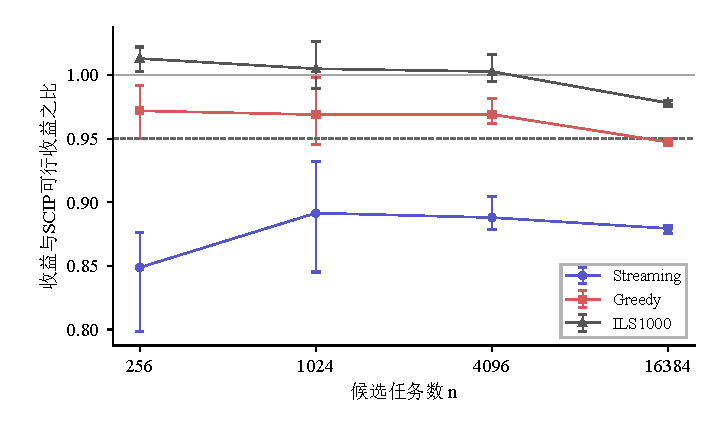
\includegraphics[width=120mm]{figures/controlled_n_quality.pdf}
 \caption{候选数各水平的质量比。点为三个结构种子的$h/L$均值，范围线为最小值至最大值，非置信区间；$L$为SCIP可行收益。虚线为$0.95$，SCIP未证明最优时比值可大于1。}
 \label{s0307:fig_n_quality}
\end{figure}

\begin{figure}[tbp]
 \centering
 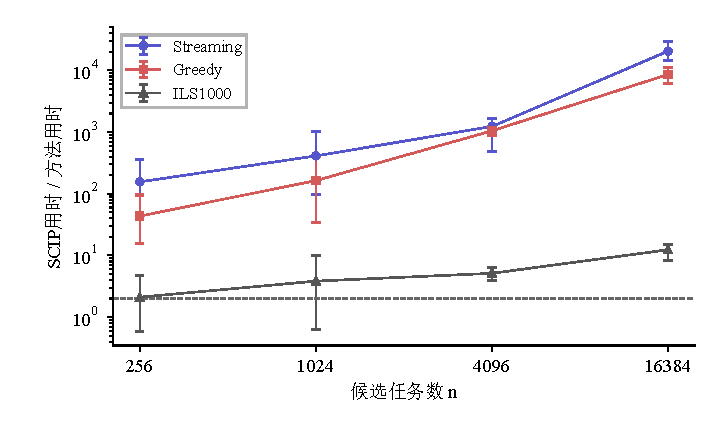
\includegraphics[width=120mm]{figures/controlled_n_time_ratio.pdf}
 \caption{候选数各水平的时间比。点为三个结构种子的$T_{\mathrm{SCIP}}/T_a$均值，范围线为最小值至最大值，非置信区间；比值大于1表示方法$a$在该条件下用时较短，虚线为2。}
 \label{s0307:fig_n_time}
\end{figure}

\paragraph{任务阶数。}
图\ref{s0307:fig_rank_quality}和图\ref{s0307:fig_rank_time}覆盖$r=4,8,16,32$。Streaming的平均质量比依次约为$0.8487$、$0.7992$、$0.7502$和$0.7054$，Greedy为$0.9718$、$0.8970$、$0.8657$和$0.8136$，ILS1000为$1.0128$、$0.9882$、$0.9694$和$0.9147$。在这组配对输入上，三种方法相对于SCIP可行值的平均质量比均随阶数水平提高而下降。

时间比却没有抵消质量损失：在$r=32$时，Streaming、Greedy和ILS1000的平均时间比分别约为11846、5984和313，但联合支持数分别为$0/3$、$0/3$和$1/3$。ILS1000在$r=8$时获得$3/3$支持，在$r=16$时降为$2/3$，在$r=32$时进一步降为$1/3$。可见，很大的时间比并不足以保证联合判据成立。这些数据揭示的是当前构造、收益与停止协议下的结果变化；它们没有单独测量内部搜索行为，不能据此认定某种未经检验的算法机制。

\begin{figure}[tbp]
 \centering
 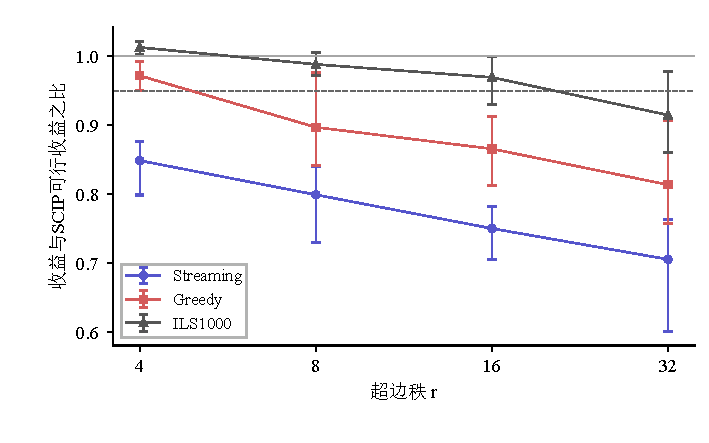
\includegraphics[width=120mm]{figures/controlled_rank_quality.pdf}
 \caption{任务阶数各水平的质量比。点为三个结构种子的$h/L$均值，范围线为最小值至最大值，非置信区间；$L$为SCIP可行收益。虚线为$0.95$，SCIP未证明最优时比值可大于1。}
 \label{s0307:fig_rank_quality}
\end{figure}

\begin{figure}[tbp]
 \centering
 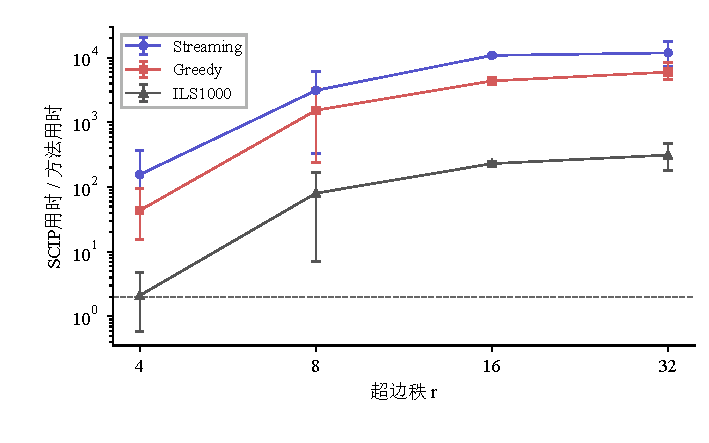
\includegraphics[width=120mm]{figures/controlled_rank_time_ratio.pdf}
 \caption{任务阶数各水平的时间比。点为三个结构种子的$T_{\mathrm{SCIP}}/T_a$均值，范围线为最小值至最大值，非置信区间；比值大于1表示方法$a$在该条件下用时较短，虚线为2。}
 \label{s0307:fig_rank_time}
\end{figure}

\paragraph{资源度。}
图\ref{s0307:fig_degree_quality}和图\ref{s0307:fig_degree_time}给出$\Delta=4,8,16,32$。Streaming平均质量比依次约为$0.8487$、$0.7620$、$0.8006$和$0.6867$，其中从8到16出现回升，不能概括为逐水平单调下降。Greedy平均质量比分别约为$0.9718$、$0.9516$、$0.9030$和$0.9200$，也存在非单调变化。虽然前节构造保证资源组粗化后的可行域嵌套，但相对于不同SCIP可行解计算的启发式质量比并无相应单调性保证。

ILS1000在$\Delta=8$和16时平均质量比分别为$0.9867$和$0.9865$，平均时间比分别为$6.8517$和$30.7168$，两个配置均获得$3/3$联合支持。到$\Delta=32$时，其平均质量比降为$0.9411$，平均时间比为$4.4089$，联合支持仅为$1/3$。从原值看，该水平的三个条件中ILS1000收益分别为510、502和478，对应SCIP收益536、527和520；时间比分布也跨越联合判据的界限。配置均值只能表达中心位置，不能替代逐种子的质量与时间配对。

\begin{figure}[tbp]
 \centering
 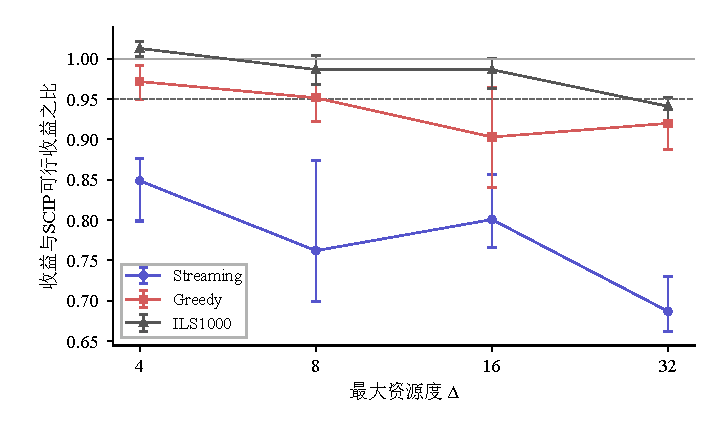
\includegraphics[width=120mm]{figures/controlled_degree_quality.pdf}
 \caption{资源度各水平的质量比。点为三个结构种子的$h/L$均值，范围线为最小值至最大值，非置信区间；$L$为SCIP可行收益。虚线为$0.95$，SCIP未证明最优时比值可大于1。}
 \label{s0307:fig_degree_quality}
\end{figure}

\begin{figure}[tbp]
 \centering
 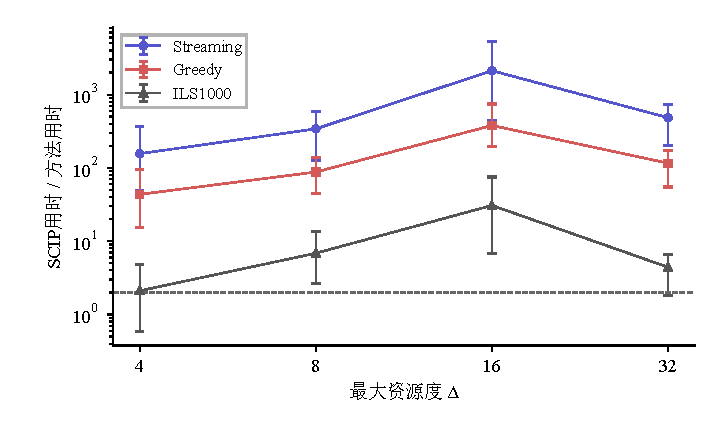
\includegraphics[width=120mm]{figures/controlled_degree_time_ratio.pdf}
 \caption{资源度各水平的时间比。点为三个结构种子的$T_{\mathrm{SCIP}}/T_a$均值，范围线为最小值至最大值，非置信区间；比值大于1表示方法$a$在该条件下用时较短，虚线为2。}
 \label{s0307:fig_degree_time}
\end{figure}

\paragraph{收益跨度。}
图\ref{s0307:fig_spread_quality}和图\ref{s0307:fig_spread_time}按$W=1,10,100,1000$展示全部水平，其中$W=100$为基准。Streaming平均质量比依次为$0.7692$、$0.8169$、$0.8487$和$0.9045$，Greedy为$0.7634$、$0.9217$、$0.9718$和$0.9785$。这两种方法在所列输入上的平均质量比随跨度增大而提高，但Streaming直到$W=1000$也仅有一个种子满足联合条件，Greedy在该水平也只有$2/3$支持。

ILS1000的平均质量比依次为$0.9764$、$1.0013$、$1.0128$和$1.0015$，对应平均时间比约为52559、$56.4644$、$2.1058$和$0.8888$。在$W=1$时，SCIP三个调用分别耗时$518.43\,\mathrm{s}$、$3163.6\,\mathrm{s}$和$3108\,\mathrm{s}$，ILS1000分别为$0.044125\,\mathrm{s}$、$0.075965\,\mathrm{s}$和$0.029804\,\mathrm{s}$，所以得到很大的时间比。到$W=1000$时，SCIP三个调用均约为$0.02\,\mathrm{s}$，ILS1000调用也处于这一量级，其时间比最大值只有$1.1823$，三个种子均未达到2。因此，ILS1000在$W=1000$虽保持或超过SCIP可行收益，联合支持仍为$0/3$。这一变化由所列收益与计时直接支持；仅凭曲线不足以进一步断定搜索树、归约作用或缓存行为的原因。

\begin{figure}[tbp]
 \centering
 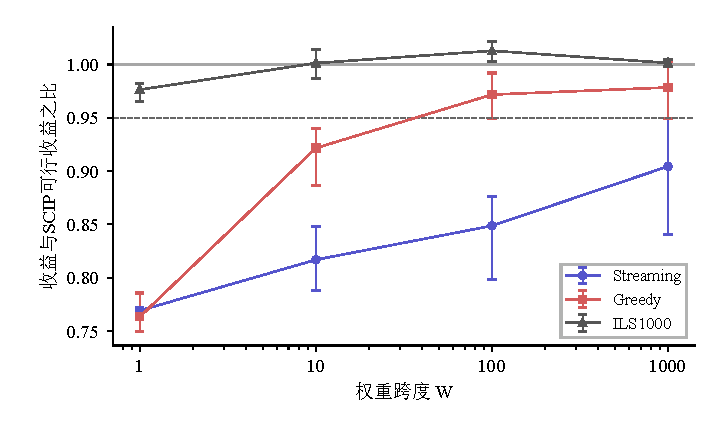
\includegraphics[width=120mm]{figures/controlled_spread_quality.pdf}
 \caption{收益跨度各水平的质量比。点为三个结构种子的$h/L$均值，范围线为最小值至最大值，非置信区间；$L$为SCIP可行收益。虚线为$0.95$，SCIP未证明最优时比值可大于1。}
 \label{s0307:fig_spread_quality}
\end{figure}

\begin{figure}[tbp]
 \centering
 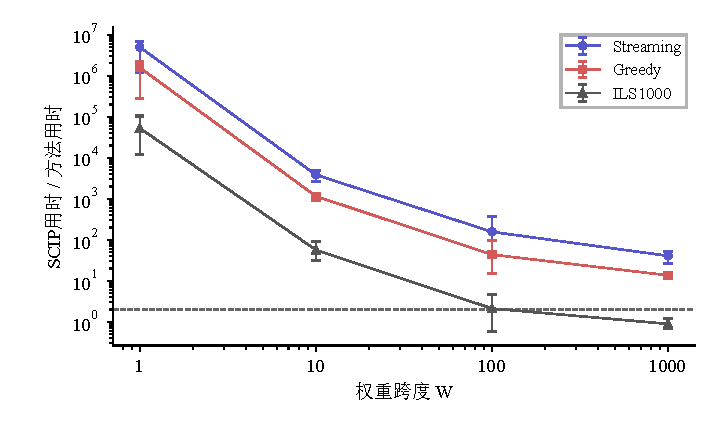
\includegraphics[width=120mm]{figures/controlled_spread_time_ratio.pdf}
 \caption{收益跨度各水平的时间比。点为三个结构种子的$T_{\mathrm{SCIP}}/T_a$均值，范围线为最小值至最大值，非置信区间；比值大于1表示方法$a$在该条件下用时较短，虚线为2。}
 \label{s0307:fig_spread_time}
\end{figure}

上述13组是既定开发条件下的完整描述。得到$3/3$支持的配置不能在观察结果后另行组成一个独立评价集；共享基准、结构种子及构造关系的配置也不能作为独立样本进行跨组显著性解释。本节不报告跨组$p$值。所有输入仍为单位容量，较大任务阶数不改变其可行域可由两两冲突表达的事实，因而这些曲线本身也不构成不可约高阶依赖或超图表示优势的证明。

\subsection{原作者完整流程的有效结果与失败分母}

原作者完整流程包含至多10轮归约、$S,\mathrm{pin}$贪心构造、ILS15和展开，不能与前述单独调用Greedy或ILS1000混为同一方法\cite{GrossmannJRS2026}。其中15是连续未改进计数的停止阈值，改进后计数重置，并非固定总迭代次数。七个既有公开输入各计划运行十个固定算法种子，共70次；实际65次有效、5次失败。表\ref{tab:author_results}同时保留计划分母、失败数以及有效输出的收益和时间统计。

{\small\setlength{\tabcolsep}{4pt}
\begin{longtable}{lrrrrrr}
\caption{公开完整流程的全部预定种子与有效子集结果}\label{tab:author_results}\\
\toprule
实例 & 有效/计划 & 失败 & 有效均值 & 有效最小 & 有效最大 & 有效均时/s\\
\midrule
\endfirsthead
\toprule
实例 & 有效/计划 & 失败 & 有效均值 & 有效最小 & 有效最大 & 有效均时/s\\
\midrule
\endhead
\midrule
\multicolumn{7}{r}{续下页}\\
\endfoot
\bottomrule
\endlastfoot
ibm01 & 10/10 & 0 & 257814 & 257521 & 258013 & 0.099067\\
ibm02 & 9/10 & 1 & 379719.3333 & 379495 & 379987 & 0.14808\\
us04 & 6/10 & 4 & 978 & 933 & 1065 & 12.339\\
bibd49 & 10/10 & 0 & 2289.9 & 2288 & 2307 & 0.022158\\
AProVE01 & 10/10 & 0 & 132908.6 & 132820 & 133005 & 0.086438\\
AProVE27 & 10/10 & 0 & 154209.6 & 154055 & 154455 & 0.071669\\
superblue19 & 10/10 & 0 & 11405360.9 & 11405242 & 11405475 & 7.9381\\
\end{longtable}
}
均值仅按有效子集计算；ibm02和us04分别有1和4个失败种子，其全十种子收益均值未定义，不能把失败计为零或删除后称完整统计。


为明确均值的适用对象，令$p$表示表中的一个公开输入，$\mathcal S_p$为其十个计划种子的集合，$\mathcal V_p\subseteq\mathcal S_p$为获得有效输出的种子集合。记$h^{\mathrm{full}}_{p,s}\geq0$为有效输出的无量纲收益，$T^{\mathrm{full}}_{p,s}>0$为对应调用时间，单位为$\mathrm{s}$。对$|\mathcal V_p|>0$的输入，表中有效均值定义为
\begin{align}
 \overline h^{\mathrm{valid}}_p
 &=\frac{1}{|\mathcal V_p|}
   \sum_{s\in\mathcal V_p}h^{\mathrm{full}}_{p,s},
 \label{s0307:author_quality_mean}\\
 \overline T^{\mathrm{valid}}_p
 &=\frac{1}{|\mathcal V_p|}
   \sum_{s\in\mathcal V_p}T^{\mathrm{full}}_{p,s}.
 \label{s0307:author_time_mean}
\end{align}
有效最小值和最大值也只在$\mathcal V_p$上取值。失败种子没有可用于上述收益平均的有效输出，不能赋零，也不能删除失败后将有效均值称为全十种子均值。

\texttt{ibm02}仅有$9/10$有效，所列379719.3333是九个有效结果的均值；\texttt{us04}仅有$6/10$有效，所列978是六个有效结果的均值。二者的全十种子收益均值均未定义。其余五个输入为$10/10$有效，才可将有效子集均值同时解释为全计划种子的均值。65次有效输出已经按原始权重和单位容量重新核验，这一事实不消除另外五次失败。

在\texttt{ibm01}上，完整流程十次收益介于257521和258013之间，均值257814，相对于SCIP最优收益265302仍少7488；有效平均调用时间为$0.099067\,\mathrm{s}$。因此，完整流程相对于Streaming收益219983有明显提高，但没有达到该输入的已知最优收益。\texttt{bibd49}的完整流程平均收益为2289.9，有效平均时间为$0.022158\,\mathrm{s}$，SCIP最优收益为2361；这同样是较短记录时间与收益差距并存的情形。

\texttt{us04}给出了不利结果：六个有效输出的收益从933到1065，最高值达到SCIP最优收益1065，但均值只有978；有效平均时间为$12.339\,\mathrm{s}$，长于SCIP历史记录的$2.5119\,\mathrm{s}$，且另外四个计划种子失败。不能只保留达到1065的输出来代表该流程。\texttt{superblue19}的十个有效输出则较集中，收益从11405242到11405475，均值11405360.9，有效平均时间为$7.9381\,\mathrm{s}$；SCIP保存的可行收益为11642395，按间隙结束。这一组记录支持对所得收益和调用成本作具体比较，但两种停止机制不同，不能扩展为统一预算下的全局优越性结论。

\subsection{三个条件上的九次停止阈值诊断}

最后考察三个既有条件上的Greedy、ILS1000和ILS5000诊断运行。三种输入分别为最大任务阶数12的1000候选合成条件、500顶点度为3的MIS转换条件，以及\texttt{ibm01}；对应编号为C06、C20和C26。各诊断调用使用算法种子0，九次输出均通过可行性核验。表\ref{s0307:tab_diagnostic}列出全部收益、选中任务数及调用时间。选中任务数是非负整数，表示二元变量中取值为1的项数，不能在非等权条件下代替收益。

\begin{table}[tbp]
 \centering
 \small
 \caption{三个既有条件的全部九次诊断运行}
 \label{s0307:tab_diagnostic}
 \begin{tabular}{llrrr}
 \toprule
 条件 & 方法 & 收益 & 选中任务数 & 时间/$\mathrm{s}$\\
 \midrule
 C06 & Greedy  & 694    & 8    & 0.0043294\\
 C06 & ILS1000 & 770    & 9    & 1.30735\\
 C06 & ILS5000 & 770    & 9    & 5.95733\\
 C20 & Greedy  & 182    & 182  & 0.0019908\\
 C20 & ILS1000 & 221    & 221  & 0.0593483\\
 C20 & ILS5000 & 222    & 222  & 0.193667\\
 C26 & Greedy  & 240686 & 4017 & 0.0301111\\
 C26 & ILS1000 & 263094 & 4085 & 33.9920\\
 C26 & ILS5000 & 264387 & 4063 & 107.008\\
 \bottomrule
 \end{tabular}
\end{table}

C06中，Greedy取得694，ILS1000提高到770，但ILS5000仍为770，调用时间却由约$1.31\,\mathrm{s}$增至$5.96\,\mathrm{s}$。因此，更大的停止阈值没有在该诊断中带来收益改进。两个ILS结果都高于初始SCIP限时收益740，这与其限时停止状态一致，不能据此宣称已知该条件最优值为770。

C20的目标为所选独立集大小，任务等权，所以收益与选中任务数相同。Greedy为182，低于初始Streaming的188；ILS1000提高到221，ILS5000进一步提高到222。与表\ref{tab:initial_results}中后续SCIP可行值221相比较，ILS5000多选了一个任务，但SCIP仍为间隙终止，222也没有因此获得最优性证明。

C26中，ILS1000从Greedy收益240686提高到263094，ILS5000进一步取得264387，但仍比SCIP最优收益265302少915。两次ILS调用分别耗时约$33.99\,\mathrm{s}$和$107.01\,\mathrm{s}$，均长于SCIP历史最优记录的$1.8463\,\mathrm{s}$。同时，ILS5000选中4063项任务，少于ILS1000的4085项，却取得更高收益；这直接说明正权加权任务选择应以权重总和评价，不能只比较接受任务数量。

ILS1000和ILS5000是分别启动的两次运行，即使使用相同算法种子，也不能未经轨迹核验就把前者视为后者的搜索前缀。阈值表示连续未改进计数，发现改进后重置，代码在计数大于阈值时停止\cite{GrossmannJRS2026}。因此，1000与5000不表示固定总迭代数，也不是相同墙钟预算。九次诊断展示了提高、保持和额外时间成本三类实际现象，支持逐输入讨论停止设置，不支持更大阈值必然改善收益或任一方法全局占优的结论。
